% Created by tikzDevice version 0.6.2-92-0ad2792 on 2013-04-07 23:51:01
% !TEX encoding = UTF-8 Unicode
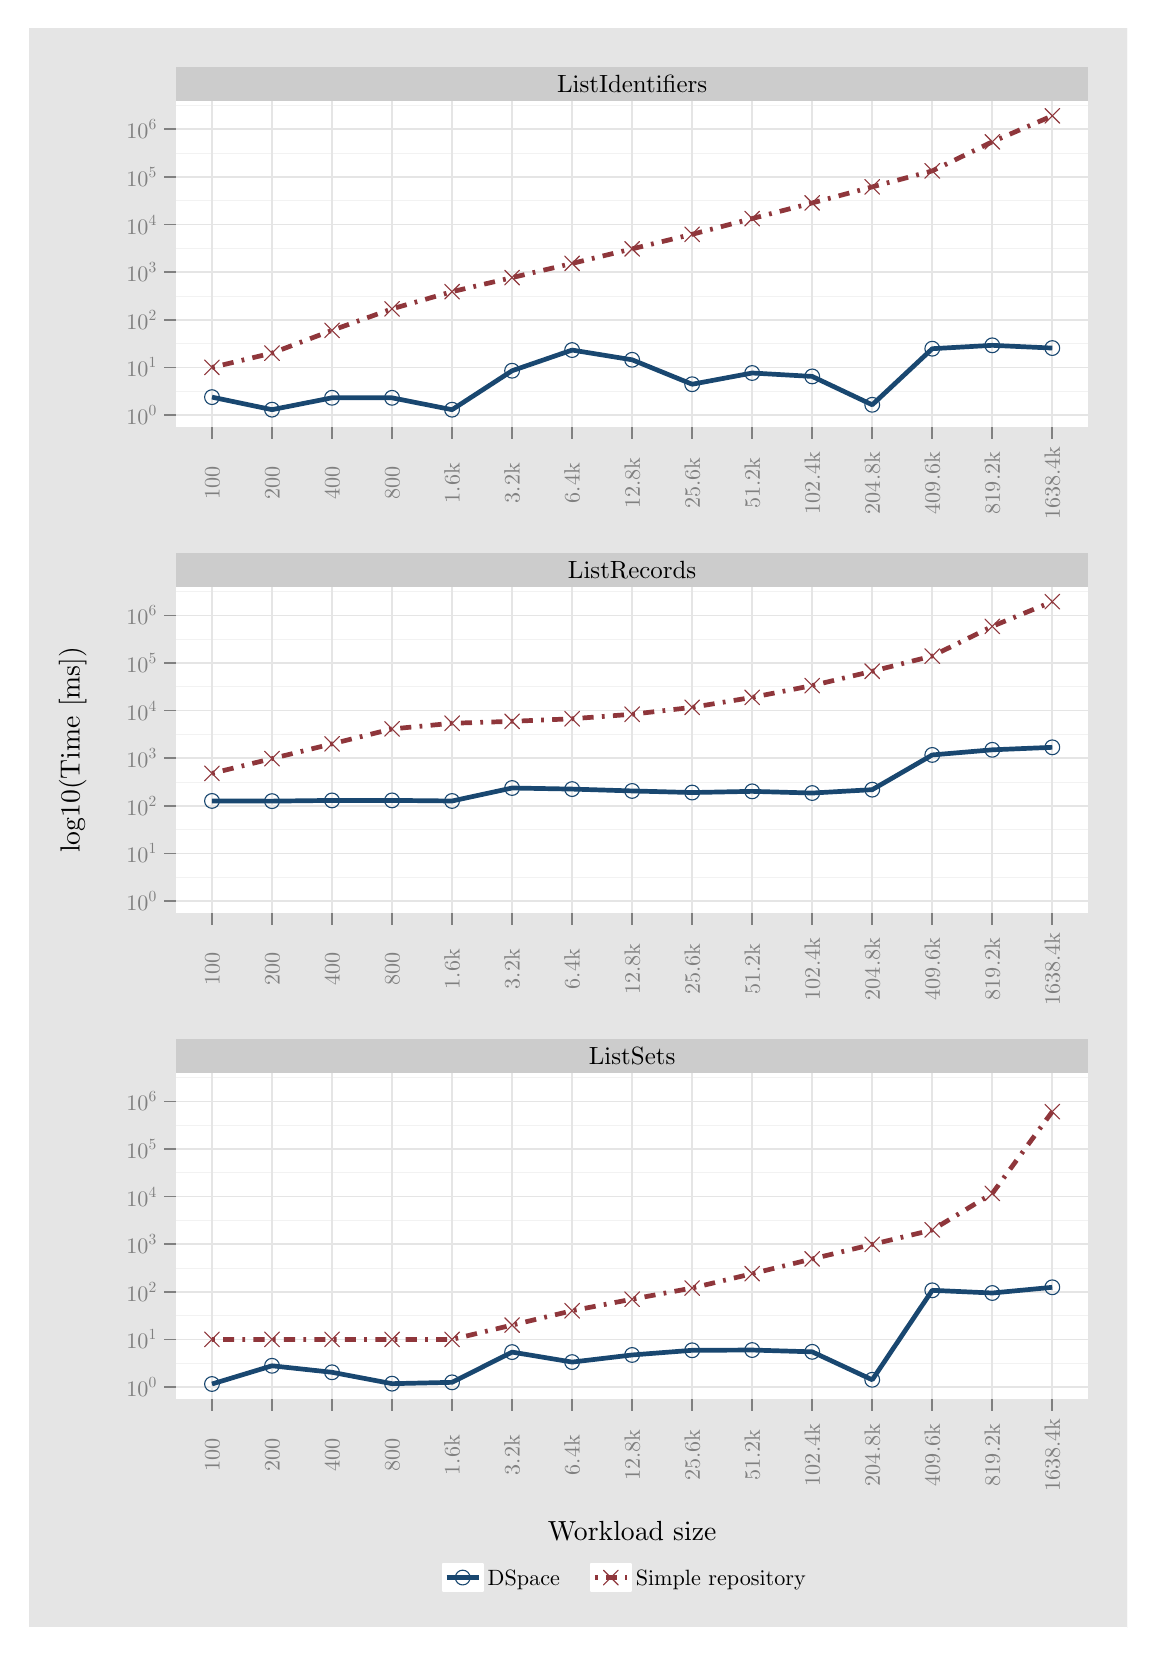
\begin{tikzpicture}[x=1pt,y=1pt]
\definecolor[named]{fillColor}{rgb}{1.00,1.00,1.00}
\path[use as bounding box,fill=fillColor,fill opacity=0.00] (0,0) rectangle (397.48,578.16);
\begin{scope}
\path[clip] (  0.00,  0.00) rectangle (397.48,578.16);
\definecolor[named]{drawColor}{rgb}{1.00,1.00,1.00}
\definecolor[named]{fillColor}{rgb}{0.90,0.90,0.90}

\path[draw=drawColor,line width= 0.6pt,line join=round,line cap=round,fill=fillColor] (  0.00,  0.00) rectangle (397.48,578.16);
\end{scope}
\begin{scope}
\path[clip] ( 53.58,433.92) rectangle (383.26,551.71);
\definecolor[named]{fillColor}{rgb}{1.00,1.00,1.00}

\path[fill=fillColor] ( 53.58,433.92) rectangle (383.26,551.71);
\definecolor[named]{drawColor}{rgb}{0.95,0.95,0.95}

\path[draw=drawColor,line width= 0.3pt,line join=round] ( 53.58,446.78) --
	(383.26,446.78);

\path[draw=drawColor,line width= 0.3pt,line join=round] ( 53.58,463.99) --
	(383.26,463.99);

\path[draw=drawColor,line width= 0.3pt,line join=round] ( 53.58,481.19) --
	(383.26,481.19);

\path[draw=drawColor,line width= 0.3pt,line join=round] ( 53.58,498.40) --
	(383.26,498.40);

\path[draw=drawColor,line width= 0.3pt,line join=round] ( 53.58,515.61) --
	(383.26,515.61);

\path[draw=drawColor,line width= 0.3pt,line join=round] ( 53.58,532.81) --
	(383.26,532.81);

\path[draw=drawColor,line width= 0.3pt,line join=round] ( 53.58,550.02) --
	(383.26,550.02);
\definecolor[named]{drawColor}{rgb}{0.90,0.90,0.90}

\path[draw=drawColor,line width= 0.6pt,line join=round] ( 53.58,438.17) --
	(383.26,438.17);

\path[draw=drawColor,line width= 0.6pt,line join=round] ( 53.58,455.38) --
	(383.26,455.38);

\path[draw=drawColor,line width= 0.6pt,line join=round] ( 53.58,472.59) --
	(383.26,472.59);

\path[draw=drawColor,line width= 0.6pt,line join=round] ( 53.58,489.80) --
	(383.26,489.80);

\path[draw=drawColor,line width= 0.6pt,line join=round] ( 53.58,507.00) --
	(383.26,507.00);

\path[draw=drawColor,line width= 0.6pt,line join=round] ( 53.58,524.21) --
	(383.26,524.21);

\path[draw=drawColor,line width= 0.6pt,line join=round] ( 53.58,541.42) --
	(383.26,541.42);

\path[draw=drawColor,line width= 0.6pt,line join=round] ( 66.60,433.92) --
	( 66.60,551.71);

\path[draw=drawColor,line width= 0.6pt,line join=round] ( 88.29,433.92) --
	( 88.29,551.71);

\path[draw=drawColor,line width= 0.6pt,line join=round] (109.97,433.92) --
	(109.97,551.71);

\path[draw=drawColor,line width= 0.6pt,line join=round] (131.66,433.92) --
	(131.66,551.71);

\path[draw=drawColor,line width= 0.6pt,line join=round] (153.35,433.92) --
	(153.35,551.71);

\path[draw=drawColor,line width= 0.6pt,line join=round] (175.04,433.92) --
	(175.04,551.71);

\path[draw=drawColor,line width= 0.6pt,line join=round] (196.73,433.92) --
	(196.73,551.71);

\path[draw=drawColor,line width= 0.6pt,line join=round] (218.42,433.92) --
	(218.42,551.71);

\path[draw=drawColor,line width= 0.6pt,line join=round] (240.11,433.92) --
	(240.11,551.71);

\path[draw=drawColor,line width= 0.6pt,line join=round] (261.80,433.92) --
	(261.80,551.71);

\path[draw=drawColor,line width= 0.6pt,line join=round] (283.49,433.92) --
	(283.49,551.71);

\path[draw=drawColor,line width= 0.6pt,line join=round] (305.18,433.92) --
	(305.18,551.71);

\path[draw=drawColor,line width= 0.6pt,line join=round] (326.87,433.92) --
	(326.87,551.71);

\path[draw=drawColor,line width= 0.6pt,line join=round] (348.56,433.92) --
	(348.56,551.71);

\path[draw=drawColor,line width= 0.6pt,line join=round] (370.25,433.92) --
	(370.25,551.71);
\definecolor[named]{drawColor}{rgb}{0.10,0.28,0.44}

\path[draw=drawColor,line width= 1.7pt,line join=round] ( 66.60,444.65) --
	( 88.29,440.12) --
	(109.97,444.41) --
	(131.66,444.40) --
	(153.35,440.11) --
	(175.04,454.19) --
	(196.73,461.66) --
	(218.42,458.14) --
	(240.11,449.31) --
	(261.80,453.37) --
	(283.49,452.13) --
	(305.18,441.88) --
	(326.87,462.15) --
	(348.56,463.37) --
	(370.25,462.38);
\definecolor[named]{drawColor}{rgb}{0.56,0.21,0.23}

\path[draw=drawColor,line width= 1.7pt,dash pattern=on 1pt off 3pt on 4pt off 3pt ,line join=round] ( 66.60,455.38) --
	( 88.29,460.56) --
	(109.97,468.77) --
	(131.66,476.55) --
	(153.35,482.76) --
	(175.04,487.84) --
	(196.73,492.97) --
	(218.42,498.23) --
	(240.11,503.49) --
	(261.80,509.18) --
	(283.49,514.82) --
	(305.18,520.62) --
	(326.87,526.39) --
	(348.56,536.92) --
	(370.25,546.30);
\definecolor[named]{drawColor}{rgb}{0.10,0.28,0.44}

\path[draw=drawColor,line width= 0.4pt,line join=round,line cap=round] ( 66.60,444.65) circle (  2.67);

\path[draw=drawColor,line width= 0.4pt,line join=round,line cap=round] ( 88.29,440.12) circle (  2.67);

\path[draw=drawColor,line width= 0.4pt,line join=round,line cap=round] (109.97,444.41) circle (  2.67);

\path[draw=drawColor,line width= 0.4pt,line join=round,line cap=round] (131.66,444.40) circle (  2.67);

\path[draw=drawColor,line width= 0.4pt,line join=round,line cap=round] (153.35,440.11) circle (  2.67);

\path[draw=drawColor,line width= 0.4pt,line join=round,line cap=round] (175.04,454.19) circle (  2.67);

\path[draw=drawColor,line width= 0.4pt,line join=round,line cap=round] (196.73,461.66) circle (  2.67);

\path[draw=drawColor,line width= 0.4pt,line join=round,line cap=round] (218.42,458.14) circle (  2.67);

\path[draw=drawColor,line width= 0.4pt,line join=round,line cap=round] (240.11,449.31) circle (  2.67);

\path[draw=drawColor,line width= 0.4pt,line join=round,line cap=round] (261.80,453.37) circle (  2.67);

\path[draw=drawColor,line width= 0.4pt,line join=round,line cap=round] (283.49,452.13) circle (  2.67);

\path[draw=drawColor,line width= 0.4pt,line join=round,line cap=round] (305.18,441.88) circle (  2.67);

\path[draw=drawColor,line width= 0.4pt,line join=round,line cap=round] (326.87,462.15) circle (  2.67);

\path[draw=drawColor,line width= 0.4pt,line join=round,line cap=round] (348.56,463.37) circle (  2.67);

\path[draw=drawColor,line width= 0.4pt,line join=round,line cap=round] (370.25,462.38) circle (  2.67);
\definecolor[named]{drawColor}{rgb}{0.56,0.21,0.23}

\path[draw=drawColor,line width= 0.4pt,line join=round,line cap=round,fill=fillColor] ( 63.93,452.71) -- ( 69.26,458.05);

\path[draw=drawColor,line width= 0.4pt,line join=round,line cap=round,fill=fillColor] ( 63.93,458.05) -- ( 69.26,452.71);

\path[draw=drawColor,line width= 0.4pt,line join=round,line cap=round,fill=fillColor] ( 85.62,457.89) -- ( 90.95,463.23);

\path[draw=drawColor,line width= 0.4pt,line join=round,line cap=round,fill=fillColor] ( 85.62,463.23) -- ( 90.95,457.89);

\path[draw=drawColor,line width= 0.4pt,line join=round,line cap=round,fill=fillColor] (107.31,466.10) -- (112.64,471.44);

\path[draw=drawColor,line width= 0.4pt,line join=round,line cap=round,fill=fillColor] (107.31,471.44) -- (112.64,466.10);

\path[draw=drawColor,line width= 0.4pt,line join=round,line cap=round,fill=fillColor] (129.00,473.89) -- (134.33,479.22);

\path[draw=drawColor,line width= 0.4pt,line join=round,line cap=round,fill=fillColor] (129.00,479.22) -- (134.33,473.89);

\path[draw=drawColor,line width= 0.4pt,line join=round,line cap=round,fill=fillColor] (150.69,480.09) -- (156.02,485.43);

\path[draw=drawColor,line width= 0.4pt,line join=round,line cap=round,fill=fillColor] (150.69,485.43) -- (156.02,480.09);

\path[draw=drawColor,line width= 0.4pt,line join=round,line cap=round,fill=fillColor] (172.37,485.18) -- (177.71,490.51);

\path[draw=drawColor,line width= 0.4pt,line join=round,line cap=round,fill=fillColor] (172.37,490.51) -- (177.71,485.18);

\path[draw=drawColor,line width= 0.4pt,line join=round,line cap=round,fill=fillColor] (194.06,490.31) -- (199.40,495.64);

\path[draw=drawColor,line width= 0.4pt,line join=round,line cap=round,fill=fillColor] (194.06,495.64) -- (199.40,490.31);

\path[draw=drawColor,line width= 0.4pt,line join=round,line cap=round,fill=fillColor] (215.75,495.56) -- (221.09,500.89);

\path[draw=drawColor,line width= 0.4pt,line join=round,line cap=round,fill=fillColor] (215.75,500.89) -- (221.09,495.56);

\path[draw=drawColor,line width= 0.4pt,line join=round,line cap=round,fill=fillColor] (237.44,500.82) -- (242.78,506.16);

\path[draw=drawColor,line width= 0.4pt,line join=round,line cap=round,fill=fillColor] (237.44,506.16) -- (242.78,500.82);

\path[draw=drawColor,line width= 0.4pt,line join=round,line cap=round,fill=fillColor] (259.13,506.51) -- (264.47,511.85);

\path[draw=drawColor,line width= 0.4pt,line join=round,line cap=round,fill=fillColor] (259.13,511.85) -- (264.47,506.51);

\path[draw=drawColor,line width= 0.4pt,line join=round,line cap=round,fill=fillColor] (280.82,512.15) -- (286.16,517.49);

\path[draw=drawColor,line width= 0.4pt,line join=round,line cap=round,fill=fillColor] (280.82,517.49) -- (286.16,512.15);

\path[draw=drawColor,line width= 0.4pt,line join=round,line cap=round,fill=fillColor] (302.51,517.95) -- (307.84,523.29);

\path[draw=drawColor,line width= 0.4pt,line join=round,line cap=round,fill=fillColor] (302.51,523.29) -- (307.84,517.95);

\path[draw=drawColor,line width= 0.4pt,line join=round,line cap=round,fill=fillColor] (324.20,523.73) -- (329.53,529.06);

\path[draw=drawColor,line width= 0.4pt,line join=round,line cap=round,fill=fillColor] (324.20,529.06) -- (329.53,523.73);

\path[draw=drawColor,line width= 0.4pt,line join=round,line cap=round,fill=fillColor] (345.89,534.26) -- (351.22,539.59);

\path[draw=drawColor,line width= 0.4pt,line join=round,line cap=round,fill=fillColor] (345.89,539.59) -- (351.22,534.26);

\path[draw=drawColor,line width= 0.4pt,line join=round,line cap=round,fill=fillColor] (367.58,543.64) -- (372.91,548.97);

\path[draw=drawColor,line width= 0.4pt,line join=round,line cap=round,fill=fillColor] (367.58,548.97) -- (372.91,543.64);
\end{scope}
\begin{scope}
\path[clip] ( 53.58,258.30) rectangle (383.26,376.10);
\definecolor[named]{fillColor}{rgb}{1.00,1.00,1.00}

\path[fill=fillColor] ( 53.58,258.30) rectangle (383.26,376.10);
\definecolor[named]{drawColor}{rgb}{0.95,0.95,0.95}

\path[draw=drawColor,line width= 0.3pt,line join=round] ( 53.58,271.17) --
	(383.26,271.17);

\path[draw=drawColor,line width= 0.3pt,line join=round] ( 53.58,288.37) --
	(383.26,288.37);

\path[draw=drawColor,line width= 0.3pt,line join=round] ( 53.58,305.58) --
	(383.26,305.58);

\path[draw=drawColor,line width= 0.3pt,line join=round] ( 53.58,322.79) --
	(383.26,322.79);

\path[draw=drawColor,line width= 0.3pt,line join=round] ( 53.58,339.99) --
	(383.26,339.99);

\path[draw=drawColor,line width= 0.3pt,line join=round] ( 53.58,357.20) --
	(383.26,357.20);

\path[draw=drawColor,line width= 0.3pt,line join=round] ( 53.58,374.41) --
	(383.26,374.41);
\definecolor[named]{drawColor}{rgb}{0.90,0.90,0.90}

\path[draw=drawColor,line width= 0.6pt,line join=round] ( 53.58,262.56) --
	(383.26,262.56);

\path[draw=drawColor,line width= 0.6pt,line join=round] ( 53.58,279.77) --
	(383.26,279.77);

\path[draw=drawColor,line width= 0.6pt,line join=round] ( 53.58,296.98) --
	(383.26,296.98);

\path[draw=drawColor,line width= 0.6pt,line join=round] ( 53.58,314.18) --
	(383.26,314.18);

\path[draw=drawColor,line width= 0.6pt,line join=round] ( 53.58,331.39) --
	(383.26,331.39);

\path[draw=drawColor,line width= 0.6pt,line join=round] ( 53.58,348.60) --
	(383.26,348.60);

\path[draw=drawColor,line width= 0.6pt,line join=round] ( 53.58,365.80) --
	(383.26,365.80);

\path[draw=drawColor,line width= 0.6pt,line join=round] ( 66.60,258.30) --
	( 66.60,376.10);

\path[draw=drawColor,line width= 0.6pt,line join=round] ( 88.29,258.30) --
	( 88.29,376.10);

\path[draw=drawColor,line width= 0.6pt,line join=round] (109.97,258.30) --
	(109.97,376.10);

\path[draw=drawColor,line width= 0.6pt,line join=round] (131.66,258.30) --
	(131.66,376.10);

\path[draw=drawColor,line width= 0.6pt,line join=round] (153.35,258.30) --
	(153.35,376.10);

\path[draw=drawColor,line width= 0.6pt,line join=round] (175.04,258.30) --
	(175.04,376.10);

\path[draw=drawColor,line width= 0.6pt,line join=round] (196.73,258.30) --
	(196.73,376.10);

\path[draw=drawColor,line width= 0.6pt,line join=round] (218.42,258.30) --
	(218.42,376.10);

\path[draw=drawColor,line width= 0.6pt,line join=round] (240.11,258.30) --
	(240.11,376.10);

\path[draw=drawColor,line width= 0.6pt,line join=round] (261.80,258.30) --
	(261.80,376.10);

\path[draw=drawColor,line width= 0.6pt,line join=round] (283.49,258.30) --
	(283.49,376.10);

\path[draw=drawColor,line width= 0.6pt,line join=round] (305.18,258.30) --
	(305.18,376.10);

\path[draw=drawColor,line width= 0.6pt,line join=round] (326.87,258.30) --
	(326.87,376.10);

\path[draw=drawColor,line width= 0.6pt,line join=round] (348.56,258.30) --
	(348.56,376.10);

\path[draw=drawColor,line width= 0.6pt,line join=round] (370.25,258.30) --
	(370.25,376.10);
\definecolor[named]{drawColor}{rgb}{0.10,0.28,0.44}

\path[draw=drawColor,line width= 1.7pt,line join=round] ( 66.60,298.74) --
	( 88.29,298.67) --
	(109.97,298.92) --
	(131.66,298.93) --
	(153.35,298.72) --
	(175.04,303.41) --
	(196.73,303.02) --
	(218.42,302.35) --
	(240.11,301.77) --
	(261.80,302.20) --
	(283.49,301.59) --
	(305.18,302.81) --
	(326.87,315.36) --
	(348.56,317.21) --
	(370.25,318.11);
\definecolor[named]{drawColor}{rgb}{0.56,0.21,0.23}

\path[draw=drawColor,line width= 1.7pt,dash pattern=on 1pt off 3pt on 4pt off 3pt ,line join=round] ( 66.60,308.70) --
	( 88.29,314.03) --
	(109.97,319.36) --
	(131.66,324.76) --
	(153.35,326.80) --
	(175.04,327.50) --
	(196.73,328.43) --
	(218.42,330.06) --
	(240.11,332.55) --
	(261.80,336.15) --
	(283.49,340.42) --
	(305.18,345.60) --
	(326.87,351.10) --
	(348.56,361.82) --
	(370.25,370.75);
\definecolor[named]{drawColor}{rgb}{0.10,0.28,0.44}

\path[draw=drawColor,line width= 0.4pt,line join=round,line cap=round] ( 66.60,298.74) circle (  2.67);

\path[draw=drawColor,line width= 0.4pt,line join=round,line cap=round] ( 88.29,298.67) circle (  2.67);

\path[draw=drawColor,line width= 0.4pt,line join=round,line cap=round] (109.97,298.92) circle (  2.67);

\path[draw=drawColor,line width= 0.4pt,line join=round,line cap=round] (131.66,298.93) circle (  2.67);

\path[draw=drawColor,line width= 0.4pt,line join=round,line cap=round] (153.35,298.72) circle (  2.67);

\path[draw=drawColor,line width= 0.4pt,line join=round,line cap=round] (175.04,303.41) circle (  2.67);

\path[draw=drawColor,line width= 0.4pt,line join=round,line cap=round] (196.73,303.02) circle (  2.67);

\path[draw=drawColor,line width= 0.4pt,line join=round,line cap=round] (218.42,302.35) circle (  2.67);

\path[draw=drawColor,line width= 0.4pt,line join=round,line cap=round] (240.11,301.77) circle (  2.67);

\path[draw=drawColor,line width= 0.4pt,line join=round,line cap=round] (261.80,302.20) circle (  2.67);

\path[draw=drawColor,line width= 0.4pt,line join=round,line cap=round] (283.49,301.59) circle (  2.67);

\path[draw=drawColor,line width= 0.4pt,line join=round,line cap=round] (305.18,302.81) circle (  2.67);

\path[draw=drawColor,line width= 0.4pt,line join=round,line cap=round] (326.87,315.36) circle (  2.67);

\path[draw=drawColor,line width= 0.4pt,line join=round,line cap=round] (348.56,317.21) circle (  2.67);

\path[draw=drawColor,line width= 0.4pt,line join=round,line cap=round] (370.25,318.11) circle (  2.67);
\definecolor[named]{drawColor}{rgb}{0.56,0.21,0.23}

\path[draw=drawColor,line width= 0.4pt,line join=round,line cap=round,fill=fillColor] ( 63.93,306.03) -- ( 69.26,311.37);

\path[draw=drawColor,line width= 0.4pt,line join=round,line cap=round,fill=fillColor] ( 63.93,311.37) -- ( 69.26,306.03);

\path[draw=drawColor,line width= 0.4pt,line join=round,line cap=round,fill=fillColor] ( 85.62,311.36) -- ( 90.95,316.70);

\path[draw=drawColor,line width= 0.4pt,line join=round,line cap=round,fill=fillColor] ( 85.62,316.70) -- ( 90.95,311.36);

\path[draw=drawColor,line width= 0.4pt,line join=round,line cap=round,fill=fillColor] (107.31,316.70) -- (112.64,322.03);

\path[draw=drawColor,line width= 0.4pt,line join=round,line cap=round,fill=fillColor] (107.31,322.03) -- (112.64,316.70);

\path[draw=drawColor,line width= 0.4pt,line join=round,line cap=round,fill=fillColor] (129.00,322.10) -- (134.33,327.43);

\path[draw=drawColor,line width= 0.4pt,line join=round,line cap=round,fill=fillColor] (129.00,327.43) -- (134.33,322.10);

\path[draw=drawColor,line width= 0.4pt,line join=round,line cap=round,fill=fillColor] (150.69,324.13) -- (156.02,329.47);

\path[draw=drawColor,line width= 0.4pt,line join=round,line cap=round,fill=fillColor] (150.69,329.47) -- (156.02,324.13);

\path[draw=drawColor,line width= 0.4pt,line join=round,line cap=round,fill=fillColor] (172.37,324.83) -- (177.71,330.17);

\path[draw=drawColor,line width= 0.4pt,line join=round,line cap=round,fill=fillColor] (172.37,330.17) -- (177.71,324.83);

\path[draw=drawColor,line width= 0.4pt,line join=round,line cap=round,fill=fillColor] (194.06,325.76) -- (199.40,331.10);

\path[draw=drawColor,line width= 0.4pt,line join=round,line cap=round,fill=fillColor] (194.06,331.10) -- (199.40,325.76);

\path[draw=drawColor,line width= 0.4pt,line join=round,line cap=round,fill=fillColor] (215.75,327.39) -- (221.09,332.73);

\path[draw=drawColor,line width= 0.4pt,line join=round,line cap=round,fill=fillColor] (215.75,332.73) -- (221.09,327.39);

\path[draw=drawColor,line width= 0.4pt,line join=round,line cap=round,fill=fillColor] (237.44,329.88) -- (242.78,335.22);

\path[draw=drawColor,line width= 0.4pt,line join=round,line cap=round,fill=fillColor] (237.44,335.22) -- (242.78,329.88);

\path[draw=drawColor,line width= 0.4pt,line join=round,line cap=round,fill=fillColor] (259.13,333.48) -- (264.47,338.81);

\path[draw=drawColor,line width= 0.4pt,line join=round,line cap=round,fill=fillColor] (259.13,338.81) -- (264.47,333.48);

\path[draw=drawColor,line width= 0.4pt,line join=round,line cap=round,fill=fillColor] (280.82,337.75) -- (286.16,343.08);

\path[draw=drawColor,line width= 0.4pt,line join=round,line cap=round,fill=fillColor] (280.82,343.08) -- (286.16,337.75);

\path[draw=drawColor,line width= 0.4pt,line join=round,line cap=round,fill=fillColor] (302.51,342.93) -- (307.84,348.27);

\path[draw=drawColor,line width= 0.4pt,line join=round,line cap=round,fill=fillColor] (302.51,348.27) -- (307.84,342.93);

\path[draw=drawColor,line width= 0.4pt,line join=round,line cap=round,fill=fillColor] (324.20,348.43) -- (329.53,353.76);

\path[draw=drawColor,line width= 0.4pt,line join=round,line cap=round,fill=fillColor] (324.20,353.76) -- (329.53,348.43);

\path[draw=drawColor,line width= 0.4pt,line join=round,line cap=round,fill=fillColor] (345.89,359.15) -- (351.22,364.48);

\path[draw=drawColor,line width= 0.4pt,line join=round,line cap=round,fill=fillColor] (345.89,364.48) -- (351.22,359.15);

\path[draw=drawColor,line width= 0.4pt,line join=round,line cap=round,fill=fillColor] (367.58,368.08) -- (372.91,373.41);

\path[draw=drawColor,line width= 0.4pt,line join=round,line cap=round,fill=fillColor] (367.58,373.41) -- (372.91,368.08);
\end{scope}
\begin{scope}
\path[clip] ( 53.58, 82.69) rectangle (383.26,200.49);
\definecolor[named]{fillColor}{rgb}{1.00,1.00,1.00}

\path[fill=fillColor] ( 53.58, 82.69) rectangle (383.26,200.49);
\definecolor[named]{drawColor}{rgb}{0.95,0.95,0.95}

\path[draw=drawColor,line width= 0.3pt,line join=round] ( 53.58, 95.55) --
	(383.26, 95.55);

\path[draw=drawColor,line width= 0.3pt,line join=round] ( 53.58,112.76) --
	(383.26,112.76);

\path[draw=drawColor,line width= 0.3pt,line join=round] ( 53.58,129.97) --
	(383.26,129.97);

\path[draw=drawColor,line width= 0.3pt,line join=round] ( 53.58,147.17) --
	(383.26,147.17);

\path[draw=drawColor,line width= 0.3pt,line join=round] ( 53.58,164.38) --
	(383.26,164.38);

\path[draw=drawColor,line width= 0.3pt,line join=round] ( 53.58,181.59) --
	(383.26,181.59);

\path[draw=drawColor,line width= 0.3pt,line join=round] ( 53.58,198.79) --
	(383.26,198.79);
\definecolor[named]{drawColor}{rgb}{0.90,0.90,0.90}

\path[draw=drawColor,line width= 0.6pt,line join=round] ( 53.58, 86.95) --
	(383.26, 86.95);

\path[draw=drawColor,line width= 0.6pt,line join=round] ( 53.58,104.16) --
	(383.26,104.16);

\path[draw=drawColor,line width= 0.6pt,line join=round] ( 53.58,121.36) --
	(383.26,121.36);

\path[draw=drawColor,line width= 0.6pt,line join=round] ( 53.58,138.57) --
	(383.26,138.57);

\path[draw=drawColor,line width= 0.6pt,line join=round] ( 53.58,155.78) --
	(383.26,155.78);

\path[draw=drawColor,line width= 0.6pt,line join=round] ( 53.58,172.98) --
	(383.26,172.98);

\path[draw=drawColor,line width= 0.6pt,line join=round] ( 53.58,190.19) --
	(383.26,190.19);

\path[draw=drawColor,line width= 0.6pt,line join=round] ( 66.60, 82.69) --
	( 66.60,200.49);

\path[draw=drawColor,line width= 0.6pt,line join=round] ( 88.29, 82.69) --
	( 88.29,200.49);

\path[draw=drawColor,line width= 0.6pt,line join=round] (109.97, 82.69) --
	(109.97,200.49);

\path[draw=drawColor,line width= 0.6pt,line join=round] (131.66, 82.69) --
	(131.66,200.49);

\path[draw=drawColor,line width= 0.6pt,line join=round] (153.35, 82.69) --
	(153.35,200.49);

\path[draw=drawColor,line width= 0.6pt,line join=round] (175.04, 82.69) --
	(175.04,200.49);

\path[draw=drawColor,line width= 0.6pt,line join=round] (196.73, 82.69) --
	(196.73,200.49);

\path[draw=drawColor,line width= 0.6pt,line join=round] (218.42, 82.69) --
	(218.42,200.49);

\path[draw=drawColor,line width= 0.6pt,line join=round] (240.11, 82.69) --
	(240.11,200.49);

\path[draw=drawColor,line width= 0.6pt,line join=round] (261.80, 82.69) --
	(261.80,200.49);

\path[draw=drawColor,line width= 0.6pt,line join=round] (283.49, 82.69) --
	(283.49,200.49);

\path[draw=drawColor,line width= 0.6pt,line join=round] (305.18, 82.69) --
	(305.18,200.49);

\path[draw=drawColor,line width= 0.6pt,line join=round] (326.87, 82.69) --
	(326.87,200.49);

\path[draw=drawColor,line width= 0.6pt,line join=round] (348.56, 82.69) --
	(348.56,200.49);

\path[draw=drawColor,line width= 0.6pt,line join=round] (370.25, 82.69) --
	(370.25,200.49);
\definecolor[named]{drawColor}{rgb}{0.10,0.28,0.44}

\path[draw=drawColor,line width= 1.7pt,line join=round] ( 66.60, 88.05) --
	( 88.29, 94.63) --
	(109.97, 92.28) --
	(131.66, 88.17) --
	(153.35, 88.65) --
	(175.04, 99.58) --
	(196.73, 95.97) --
	(218.42, 98.54) --
	(240.11,100.23) --
	(261.80,100.32) --
	(283.49, 99.67) --
	(305.18, 89.57) --
	(326.87,121.90) --
	(348.56,120.93) --
	(370.25,122.99);
\definecolor[named]{drawColor}{rgb}{0.56,0.21,0.23}

\path[draw=drawColor,line width= 1.7pt,dash pattern=on 1pt off 3pt on 4pt off 3pt ,line join=round] ( 66.60,104.16) --
	( 88.29,104.16) --
	(109.97,104.16) --
	(131.66,104.16) --
	(153.35,104.16) --
	(175.04,109.34) --
	(196.73,114.52) --
	(218.42,118.70) --
	(240.11,122.73) --
	(261.80,127.91) --
	(283.49,133.24) --
	(305.18,138.49) --
	(326.87,143.71) --
	(348.56,156.89) --
	(370.25,186.49);
\definecolor[named]{drawColor}{rgb}{0.10,0.28,0.44}

\path[draw=drawColor,line width= 0.4pt,line join=round,line cap=round] ( 66.60, 88.05) circle (  2.67);

\path[draw=drawColor,line width= 0.4pt,line join=round,line cap=round] ( 88.29, 94.63) circle (  2.67);

\path[draw=drawColor,line width= 0.4pt,line join=round,line cap=round] (109.97, 92.28) circle (  2.67);

\path[draw=drawColor,line width= 0.4pt,line join=round,line cap=round] (131.66, 88.17) circle (  2.67);

\path[draw=drawColor,line width= 0.4pt,line join=round,line cap=round] (153.35, 88.65) circle (  2.67);

\path[draw=drawColor,line width= 0.4pt,line join=round,line cap=round] (175.04, 99.58) circle (  2.67);

\path[draw=drawColor,line width= 0.4pt,line join=round,line cap=round] (196.73, 95.97) circle (  2.67);

\path[draw=drawColor,line width= 0.4pt,line join=round,line cap=round] (218.42, 98.54) circle (  2.67);

\path[draw=drawColor,line width= 0.4pt,line join=round,line cap=round] (240.11,100.23) circle (  2.67);

\path[draw=drawColor,line width= 0.4pt,line join=round,line cap=round] (261.80,100.32) circle (  2.67);

\path[draw=drawColor,line width= 0.4pt,line join=round,line cap=round] (283.49, 99.67) circle (  2.67);

\path[draw=drawColor,line width= 0.4pt,line join=round,line cap=round] (305.18, 89.57) circle (  2.67);

\path[draw=drawColor,line width= 0.4pt,line join=round,line cap=round] (326.87,121.90) circle (  2.67);

\path[draw=drawColor,line width= 0.4pt,line join=round,line cap=round] (348.56,120.93) circle (  2.67);

\path[draw=drawColor,line width= 0.4pt,line join=round,line cap=round] (370.25,122.99) circle (  2.67);
\definecolor[named]{drawColor}{rgb}{0.56,0.21,0.23}

\path[draw=drawColor,line width= 0.4pt,line join=round,line cap=round,fill=fillColor] ( 63.93,101.49) -- ( 69.26,106.82);

\path[draw=drawColor,line width= 0.4pt,line join=round,line cap=round,fill=fillColor] ( 63.93,106.82) -- ( 69.26,101.49);

\path[draw=drawColor,line width= 0.4pt,line join=round,line cap=round,fill=fillColor] ( 85.62,101.49) -- ( 90.95,106.82);

\path[draw=drawColor,line width= 0.4pt,line join=round,line cap=round,fill=fillColor] ( 85.62,106.82) -- ( 90.95,101.49);

\path[draw=drawColor,line width= 0.4pt,line join=round,line cap=round,fill=fillColor] (107.31,101.49) -- (112.64,106.82);

\path[draw=drawColor,line width= 0.4pt,line join=round,line cap=round,fill=fillColor] (107.31,106.82) -- (112.64,101.49);

\path[draw=drawColor,line width= 0.4pt,line join=round,line cap=round,fill=fillColor] (129.00,101.49) -- (134.33,106.82);

\path[draw=drawColor,line width= 0.4pt,line join=round,line cap=round,fill=fillColor] (129.00,106.82) -- (134.33,101.49);

\path[draw=drawColor,line width= 0.4pt,line join=round,line cap=round,fill=fillColor] (150.69,101.49) -- (156.02,106.82);

\path[draw=drawColor,line width= 0.4pt,line join=round,line cap=round,fill=fillColor] (150.69,106.82) -- (156.02,101.49);

\path[draw=drawColor,line width= 0.4pt,line join=round,line cap=round,fill=fillColor] (172.37,106.67) -- (177.71,112.00);

\path[draw=drawColor,line width= 0.4pt,line join=round,line cap=round,fill=fillColor] (172.37,112.00) -- (177.71,106.67);

\path[draw=drawColor,line width= 0.4pt,line join=round,line cap=round,fill=fillColor] (194.06,111.85) -- (199.40,117.18);

\path[draw=drawColor,line width= 0.4pt,line join=round,line cap=round,fill=fillColor] (194.06,117.18) -- (199.40,111.85);

\path[draw=drawColor,line width= 0.4pt,line join=round,line cap=round,fill=fillColor] (215.75,116.03) -- (221.09,121.37);

\path[draw=drawColor,line width= 0.4pt,line join=round,line cap=round,fill=fillColor] (215.75,121.37) -- (221.09,116.03);

\path[draw=drawColor,line width= 0.4pt,line join=round,line cap=round,fill=fillColor] (237.44,120.06) -- (242.78,125.39);

\path[draw=drawColor,line width= 0.4pt,line join=round,line cap=round,fill=fillColor] (237.44,125.39) -- (242.78,120.06);

\path[draw=drawColor,line width= 0.4pt,line join=round,line cap=round,fill=fillColor] (259.13,125.24) -- (264.47,130.57);

\path[draw=drawColor,line width= 0.4pt,line join=round,line cap=round,fill=fillColor] (259.13,130.57) -- (264.47,125.24);

\path[draw=drawColor,line width= 0.4pt,line join=round,line cap=round,fill=fillColor] (280.82,130.57) -- (286.16,135.91);

\path[draw=drawColor,line width= 0.4pt,line join=round,line cap=round,fill=fillColor] (280.82,135.91) -- (286.16,130.57);

\path[draw=drawColor,line width= 0.4pt,line join=round,line cap=round,fill=fillColor] (302.51,135.83) -- (307.84,141.16);

\path[draw=drawColor,line width= 0.4pt,line join=round,line cap=round,fill=fillColor] (302.51,141.16) -- (307.84,135.83);

\path[draw=drawColor,line width= 0.4pt,line join=round,line cap=round,fill=fillColor] (324.20,141.05) -- (329.53,146.38);

\path[draw=drawColor,line width= 0.4pt,line join=round,line cap=round,fill=fillColor] (324.20,146.38) -- (329.53,141.05);

\path[draw=drawColor,line width= 0.4pt,line join=round,line cap=round,fill=fillColor] (345.89,154.23) -- (351.22,159.56);

\path[draw=drawColor,line width= 0.4pt,line join=round,line cap=round,fill=fillColor] (345.89,159.56) -- (351.22,154.23);

\path[draw=drawColor,line width= 0.4pt,line join=round,line cap=round,fill=fillColor] (367.58,183.82) -- (372.91,189.15);

\path[draw=drawColor,line width= 0.4pt,line join=round,line cap=round,fill=fillColor] (367.58,189.15) -- (372.91,183.82);
\end{scope}
\begin{scope}
\path[clip] (  0.00,  0.00) rectangle (397.48,578.16);
\definecolor[named]{fillColor}{rgb}{0.80,0.80,0.80}

\path[fill=fillColor] ( 53.58,551.71) rectangle (383.26,563.93);
\definecolor[named]{drawColor}{rgb}{0.00,0.00,0.00}

\node[text=drawColor,anchor=base,inner sep=0pt, outer sep=0pt, scale=  0.90] at (218.42,554.72) {ListIdentifiers};
\end{scope}
\begin{scope}
\path[clip] (  0.00,  0.00) rectangle (397.48,578.16);
\definecolor[named]{fillColor}{rgb}{0.80,0.80,0.80}

\path[fill=fillColor] ( 53.58,376.10) rectangle (383.26,388.32);
\definecolor[named]{drawColor}{rgb}{0.00,0.00,0.00}

\node[text=drawColor,anchor=base,inner sep=0pt, outer sep=0pt, scale=  0.90] at (218.42,379.11) {ListRecords};
\end{scope}
\begin{scope}
\path[clip] (  0.00,  0.00) rectangle (397.48,578.16);
\definecolor[named]{fillColor}{rgb}{0.80,0.80,0.80}

\path[fill=fillColor] ( 53.58,200.49) rectangle (383.26,212.71);
\definecolor[named]{drawColor}{rgb}{0.00,0.00,0.00}

\node[text=drawColor,anchor=base,inner sep=0pt, outer sep=0pt, scale=  0.90] at (218.42,203.50) {ListSets};
\end{scope}
\begin{scope}
\path[clip] (  0.00,  0.00) rectangle (397.48,578.16);
\definecolor[named]{drawColor}{rgb}{0.50,0.50,0.50}

\node[text=drawColor,anchor=base west,inner sep=0pt, outer sep=0pt, scale=  0.80] at ( 35.67,434.74) {10};

\node[text=drawColor,anchor=base west,inner sep=0pt, outer sep=0pt, scale=  0.56] at ( 43.67,438.01) {0};

\node[text=drawColor,anchor=base west,inner sep=0pt, outer sep=0pt, scale=  0.80] at ( 35.67,451.95) {10};

\node[text=drawColor,anchor=base west,inner sep=0pt, outer sep=0pt, scale=  0.56] at ( 43.67,455.22) {1};

\node[text=drawColor,anchor=base west,inner sep=0pt, outer sep=0pt, scale=  0.80] at ( 35.67,469.16) {10};

\node[text=drawColor,anchor=base west,inner sep=0pt, outer sep=0pt, scale=  0.56] at ( 43.67,472.43) {2};

\node[text=drawColor,anchor=base west,inner sep=0pt, outer sep=0pt, scale=  0.80] at ( 35.67,486.36) {10};

\node[text=drawColor,anchor=base west,inner sep=0pt, outer sep=0pt, scale=  0.56] at ( 43.67,489.64) {3};

\node[text=drawColor,anchor=base west,inner sep=0pt, outer sep=0pt, scale=  0.80] at ( 35.67,503.57) {10};

\node[text=drawColor,anchor=base west,inner sep=0pt, outer sep=0pt, scale=  0.56] at ( 43.67,506.84) {4};

\node[text=drawColor,anchor=base west,inner sep=0pt, outer sep=0pt, scale=  0.80] at ( 35.67,520.78) {10};

\node[text=drawColor,anchor=base west,inner sep=0pt, outer sep=0pt, scale=  0.56] at ( 43.67,524.05) {5};

\node[text=drawColor,anchor=base west,inner sep=0pt, outer sep=0pt, scale=  0.80] at ( 35.67,537.99) {10};

\node[text=drawColor,anchor=base west,inner sep=0pt, outer sep=0pt, scale=  0.56] at ( 43.67,541.26) {6};
\end{scope}
\begin{scope}
\path[clip] (  0.00,  0.00) rectangle (397.48,578.16);
\definecolor[named]{drawColor}{rgb}{0.50,0.50,0.50}

\path[draw=drawColor,line width= 0.6pt,line join=round] ( 49.31,438.17) --
	( 53.58,438.17);

\path[draw=drawColor,line width= 0.6pt,line join=round] ( 49.31,455.38) --
	( 53.58,455.38);

\path[draw=drawColor,line width= 0.6pt,line join=round] ( 49.31,472.59) --
	( 53.58,472.59);

\path[draw=drawColor,line width= 0.6pt,line join=round] ( 49.31,489.80) --
	( 53.58,489.80);

\path[draw=drawColor,line width= 0.6pt,line join=round] ( 49.31,507.00) --
	( 53.58,507.00);

\path[draw=drawColor,line width= 0.6pt,line join=round] ( 49.31,524.21) --
	( 53.58,524.21);

\path[draw=drawColor,line width= 0.6pt,line join=round] ( 49.31,541.42) --
	( 53.58,541.42);
\end{scope}
\begin{scope}
\path[clip] (  0.00,  0.00) rectangle (397.48,578.16);
\definecolor[named]{drawColor}{rgb}{0.50,0.50,0.50}

\node[text=drawColor,anchor=base west,inner sep=0pt, outer sep=0pt, scale=  0.80] at ( 35.67,259.13) {10};

\node[text=drawColor,anchor=base west,inner sep=0pt, outer sep=0pt, scale=  0.56] at ( 43.67,262.40) {0};

\node[text=drawColor,anchor=base west,inner sep=0pt, outer sep=0pt, scale=  0.80] at ( 35.67,276.34) {10};

\node[text=drawColor,anchor=base west,inner sep=0pt, outer sep=0pt, scale=  0.56] at ( 43.67,279.61) {1};

\node[text=drawColor,anchor=base west,inner sep=0pt, outer sep=0pt, scale=  0.80] at ( 35.67,293.54) {10};

\node[text=drawColor,anchor=base west,inner sep=0pt, outer sep=0pt, scale=  0.56] at ( 43.67,296.82) {2};

\node[text=drawColor,anchor=base west,inner sep=0pt, outer sep=0pt, scale=  0.80] at ( 35.67,310.75) {10};

\node[text=drawColor,anchor=base west,inner sep=0pt, outer sep=0pt, scale=  0.56] at ( 43.67,314.02) {3};

\node[text=drawColor,anchor=base west,inner sep=0pt, outer sep=0pt, scale=  0.80] at ( 35.67,327.96) {10};

\node[text=drawColor,anchor=base west,inner sep=0pt, outer sep=0pt, scale=  0.56] at ( 43.67,331.23) {4};

\node[text=drawColor,anchor=base west,inner sep=0pt, outer sep=0pt, scale=  0.80] at ( 35.67,345.17) {10};

\node[text=drawColor,anchor=base west,inner sep=0pt, outer sep=0pt, scale=  0.56] at ( 43.67,348.44) {5};

\node[text=drawColor,anchor=base west,inner sep=0pt, outer sep=0pt, scale=  0.80] at ( 35.67,362.37) {10};

\node[text=drawColor,anchor=base west,inner sep=0pt, outer sep=0pt, scale=  0.56] at ( 43.67,365.64) {6};
\end{scope}
\begin{scope}
\path[clip] (  0.00,  0.00) rectangle (397.48,578.16);
\definecolor[named]{drawColor}{rgb}{0.50,0.50,0.50}

\path[draw=drawColor,line width= 0.6pt,line join=round] ( 49.31,262.56) --
	( 53.58,262.56);

\path[draw=drawColor,line width= 0.6pt,line join=round] ( 49.31,279.77) --
	( 53.58,279.77);

\path[draw=drawColor,line width= 0.6pt,line join=round] ( 49.31,296.98) --
	( 53.58,296.98);

\path[draw=drawColor,line width= 0.6pt,line join=round] ( 49.31,314.18) --
	( 53.58,314.18);

\path[draw=drawColor,line width= 0.6pt,line join=round] ( 49.31,331.39) --
	( 53.58,331.39);

\path[draw=drawColor,line width= 0.6pt,line join=round] ( 49.31,348.60) --
	( 53.58,348.60);

\path[draw=drawColor,line width= 0.6pt,line join=round] ( 49.31,365.80) --
	( 53.58,365.80);
\end{scope}
\begin{scope}
\path[clip] (  0.00,  0.00) rectangle (397.48,578.16);
\definecolor[named]{drawColor}{rgb}{0.50,0.50,0.50}

\node[text=drawColor,anchor=base west,inner sep=0pt, outer sep=0pt, scale=  0.80] at ( 35.67, 83.52) {10};

\node[text=drawColor,anchor=base west,inner sep=0pt, outer sep=0pt, scale=  0.56] at ( 43.67, 86.79) {0};

\node[text=drawColor,anchor=base west,inner sep=0pt, outer sep=0pt, scale=  0.80] at ( 35.67,100.72) {10};

\node[text=drawColor,anchor=base west,inner sep=0pt, outer sep=0pt, scale=  0.56] at ( 43.67,104.00) {1};

\node[text=drawColor,anchor=base west,inner sep=0pt, outer sep=0pt, scale=  0.80] at ( 35.67,117.93) {10};

\node[text=drawColor,anchor=base west,inner sep=0pt, outer sep=0pt, scale=  0.56] at ( 43.67,121.20) {2};

\node[text=drawColor,anchor=base west,inner sep=0pt, outer sep=0pt, scale=  0.80] at ( 35.67,135.14) {10};

\node[text=drawColor,anchor=base west,inner sep=0pt, outer sep=0pt, scale=  0.56] at ( 43.67,138.41) {3};

\node[text=drawColor,anchor=base west,inner sep=0pt, outer sep=0pt, scale=  0.80] at ( 35.67,152.35) {10};

\node[text=drawColor,anchor=base west,inner sep=0pt, outer sep=0pt, scale=  0.56] at ( 43.67,155.62) {4};

\node[text=drawColor,anchor=base west,inner sep=0pt, outer sep=0pt, scale=  0.80] at ( 35.67,169.55) {10};

\node[text=drawColor,anchor=base west,inner sep=0pt, outer sep=0pt, scale=  0.56] at ( 43.67,172.82) {5};

\node[text=drawColor,anchor=base west,inner sep=0pt, outer sep=0pt, scale=  0.80] at ( 35.67,186.76) {10};

\node[text=drawColor,anchor=base west,inner sep=0pt, outer sep=0pt, scale=  0.56] at ( 43.67,190.03) {6};
\end{scope}
\begin{scope}
\path[clip] (  0.00,  0.00) rectangle (397.48,578.16);
\definecolor[named]{drawColor}{rgb}{0.50,0.50,0.50}

\path[draw=drawColor,line width= 0.6pt,line join=round] ( 49.31, 86.95) --
	( 53.58, 86.95);

\path[draw=drawColor,line width= 0.6pt,line join=round] ( 49.31,104.16) --
	( 53.58,104.16);

\path[draw=drawColor,line width= 0.6pt,line join=round] ( 49.31,121.36) --
	( 53.58,121.36);

\path[draw=drawColor,line width= 0.6pt,line join=round] ( 49.31,138.57) --
	( 53.58,138.57);

\path[draw=drawColor,line width= 0.6pt,line join=round] ( 49.31,155.78) --
	( 53.58,155.78);

\path[draw=drawColor,line width= 0.6pt,line join=round] ( 49.31,172.98) --
	( 53.58,172.98);

\path[draw=drawColor,line width= 0.6pt,line join=round] ( 49.31,190.19) --
	( 53.58,190.19);
\end{scope}
\begin{scope}
\path[clip] (  0.00,  0.00) rectangle (397.48,578.16);
\definecolor[named]{drawColor}{rgb}{0.50,0.50,0.50}

\path[draw=drawColor,line width= 0.6pt,line join=round] ( 66.60,429.65) --
	( 66.60,433.92);

\path[draw=drawColor,line width= 0.6pt,line join=round] ( 88.29,429.65) --
	( 88.29,433.92);

\path[draw=drawColor,line width= 0.6pt,line join=round] (109.97,429.65) --
	(109.97,433.92);

\path[draw=drawColor,line width= 0.6pt,line join=round] (131.66,429.65) --
	(131.66,433.92);

\path[draw=drawColor,line width= 0.6pt,line join=round] (153.35,429.65) --
	(153.35,433.92);

\path[draw=drawColor,line width= 0.6pt,line join=round] (175.04,429.65) --
	(175.04,433.92);

\path[draw=drawColor,line width= 0.6pt,line join=round] (196.73,429.65) --
	(196.73,433.92);

\path[draw=drawColor,line width= 0.6pt,line join=round] (218.42,429.65) --
	(218.42,433.92);

\path[draw=drawColor,line width= 0.6pt,line join=round] (240.11,429.65) --
	(240.11,433.92);

\path[draw=drawColor,line width= 0.6pt,line join=round] (261.80,429.65) --
	(261.80,433.92);

\path[draw=drawColor,line width= 0.6pt,line join=round] (283.49,429.65) --
	(283.49,433.92);

\path[draw=drawColor,line width= 0.6pt,line join=round] (305.18,429.65) --
	(305.18,433.92);

\path[draw=drawColor,line width= 0.6pt,line join=round] (326.87,429.65) --
	(326.87,433.92);

\path[draw=drawColor,line width= 0.6pt,line join=round] (348.56,429.65) --
	(348.56,433.92);

\path[draw=drawColor,line width= 0.6pt,line join=round] (370.25,429.65) --
	(370.25,433.92);
\end{scope}
\begin{scope}
\path[clip] (  0.00,  0.00) rectangle (397.48,578.16);
\definecolor[named]{drawColor}{rgb}{0.50,0.50,0.50}

\node[text=drawColor,rotate= 90.00,anchor=base,inner sep=0pt, outer sep=0pt, scale=  0.80] at ( 69.35,413.58) {100};

\node[text=drawColor,rotate= 90.00,anchor=base,inner sep=0pt, outer sep=0pt, scale=  0.80] at ( 91.04,413.58) {200};

\node[text=drawColor,rotate= 90.00,anchor=base,inner sep=0pt, outer sep=0pt, scale=  0.80] at (112.73,413.58) {400};

\node[text=drawColor,rotate= 90.00,anchor=base,inner sep=0pt, outer sep=0pt, scale=  0.80] at (134.42,413.58) {800};

\node[text=drawColor,rotate= 90.00,anchor=base,inner sep=0pt, outer sep=0pt, scale=  0.80] at (156.11,413.58) {1.6k};

\node[text=drawColor,rotate= 90.00,anchor=base,inner sep=0pt, outer sep=0pt, scale=  0.80] at (177.80,413.58) {3.2k};

\node[text=drawColor,rotate= 90.00,anchor=base,inner sep=0pt, outer sep=0pt, scale=  0.80] at (199.49,413.58) {6.4k};

\node[text=drawColor,rotate= 90.00,anchor=base,inner sep=0pt, outer sep=0pt, scale=  0.80] at (221.18,413.58) {12.8k};

\node[text=drawColor,rotate= 90.00,anchor=base,inner sep=0pt, outer sep=0pt, scale=  0.80] at (242.86,413.58) {25.6k};

\node[text=drawColor,rotate= 90.00,anchor=base,inner sep=0pt, outer sep=0pt, scale=  0.80] at (264.55,413.58) {51.2k};

\node[text=drawColor,rotate= 90.00,anchor=base,inner sep=0pt, outer sep=0pt, scale=  0.80] at (286.24,413.58) {102.4k};

\node[text=drawColor,rotate= 90.00,anchor=base,inner sep=0pt, outer sep=0pt, scale=  0.80] at (307.93,413.58) {204.8k};

\node[text=drawColor,rotate= 90.00,anchor=base,inner sep=0pt, outer sep=0pt, scale=  0.80] at (329.62,413.58) {409.6k};

\node[text=drawColor,rotate= 90.00,anchor=base,inner sep=0pt, outer sep=0pt, scale=  0.80] at (351.31,413.58) {819.2k};

\node[text=drawColor,rotate= 90.00,anchor=base,inner sep=0pt, outer sep=0pt, scale=  0.80] at (373.00,413.58) {1638.4k};
\end{scope}
\begin{scope}
\path[clip] (  0.00,  0.00) rectangle (397.48,578.16);
\definecolor[named]{drawColor}{rgb}{0.50,0.50,0.50}

\path[draw=drawColor,line width= 0.6pt,line join=round] ( 66.60,254.04) --
	( 66.60,258.30);

\path[draw=drawColor,line width= 0.6pt,line join=round] ( 88.29,254.04) --
	( 88.29,258.30);

\path[draw=drawColor,line width= 0.6pt,line join=round] (109.97,254.04) --
	(109.97,258.30);

\path[draw=drawColor,line width= 0.6pt,line join=round] (131.66,254.04) --
	(131.66,258.30);

\path[draw=drawColor,line width= 0.6pt,line join=round] (153.35,254.04) --
	(153.35,258.30);

\path[draw=drawColor,line width= 0.6pt,line join=round] (175.04,254.04) --
	(175.04,258.30);

\path[draw=drawColor,line width= 0.6pt,line join=round] (196.73,254.04) --
	(196.73,258.30);

\path[draw=drawColor,line width= 0.6pt,line join=round] (218.42,254.04) --
	(218.42,258.30);

\path[draw=drawColor,line width= 0.6pt,line join=round] (240.11,254.04) --
	(240.11,258.30);

\path[draw=drawColor,line width= 0.6pt,line join=round] (261.80,254.04) --
	(261.80,258.30);

\path[draw=drawColor,line width= 0.6pt,line join=round] (283.49,254.04) --
	(283.49,258.30);

\path[draw=drawColor,line width= 0.6pt,line join=round] (305.18,254.04) --
	(305.18,258.30);

\path[draw=drawColor,line width= 0.6pt,line join=round] (326.87,254.04) --
	(326.87,258.30);

\path[draw=drawColor,line width= 0.6pt,line join=round] (348.56,254.04) --
	(348.56,258.30);

\path[draw=drawColor,line width= 0.6pt,line join=round] (370.25,254.04) --
	(370.25,258.30);
\end{scope}
\begin{scope}
\path[clip] (  0.00,  0.00) rectangle (397.48,578.16);
\definecolor[named]{drawColor}{rgb}{0.50,0.50,0.50}

\node[text=drawColor,rotate= 90.00,anchor=base,inner sep=0pt, outer sep=0pt, scale=  0.80] at ( 69.35,237.97) {100};

\node[text=drawColor,rotate= 90.00,anchor=base,inner sep=0pt, outer sep=0pt, scale=  0.80] at ( 91.04,237.97) {200};

\node[text=drawColor,rotate= 90.00,anchor=base,inner sep=0pt, outer sep=0pt, scale=  0.80] at (112.73,237.97) {400};

\node[text=drawColor,rotate= 90.00,anchor=base,inner sep=0pt, outer sep=0pt, scale=  0.80] at (134.42,237.97) {800};

\node[text=drawColor,rotate= 90.00,anchor=base,inner sep=0pt, outer sep=0pt, scale=  0.80] at (156.11,237.97) {1.6k};

\node[text=drawColor,rotate= 90.00,anchor=base,inner sep=0pt, outer sep=0pt, scale=  0.80] at (177.80,237.97) {3.2k};

\node[text=drawColor,rotate= 90.00,anchor=base,inner sep=0pt, outer sep=0pt, scale=  0.80] at (199.49,237.97) {6.4k};

\node[text=drawColor,rotate= 90.00,anchor=base,inner sep=0pt, outer sep=0pt, scale=  0.80] at (221.18,237.97) {12.8k};

\node[text=drawColor,rotate= 90.00,anchor=base,inner sep=0pt, outer sep=0pt, scale=  0.80] at (242.86,237.97) {25.6k};

\node[text=drawColor,rotate= 90.00,anchor=base,inner sep=0pt, outer sep=0pt, scale=  0.80] at (264.55,237.97) {51.2k};

\node[text=drawColor,rotate= 90.00,anchor=base,inner sep=0pt, outer sep=0pt, scale=  0.80] at (286.24,237.97) {102.4k};

\node[text=drawColor,rotate= 90.00,anchor=base,inner sep=0pt, outer sep=0pt, scale=  0.80] at (307.93,237.97) {204.8k};

\node[text=drawColor,rotate= 90.00,anchor=base,inner sep=0pt, outer sep=0pt, scale=  0.80] at (329.62,237.97) {409.6k};

\node[text=drawColor,rotate= 90.00,anchor=base,inner sep=0pt, outer sep=0pt, scale=  0.80] at (351.31,237.97) {819.2k};

\node[text=drawColor,rotate= 90.00,anchor=base,inner sep=0pt, outer sep=0pt, scale=  0.80] at (373.00,237.97) {1638.4k};
\end{scope}
\begin{scope}
\path[clip] (  0.00,  0.00) rectangle (397.48,578.16);
\definecolor[named]{drawColor}{rgb}{0.50,0.50,0.50}

\path[draw=drawColor,line width= 0.6pt,line join=round] ( 66.60, 78.42) --
	( 66.60, 82.69);

\path[draw=drawColor,line width= 0.6pt,line join=round] ( 88.29, 78.42) --
	( 88.29, 82.69);

\path[draw=drawColor,line width= 0.6pt,line join=round] (109.97, 78.42) --
	(109.97, 82.69);

\path[draw=drawColor,line width= 0.6pt,line join=round] (131.66, 78.42) --
	(131.66, 82.69);

\path[draw=drawColor,line width= 0.6pt,line join=round] (153.35, 78.42) --
	(153.35, 82.69);

\path[draw=drawColor,line width= 0.6pt,line join=round] (175.04, 78.42) --
	(175.04, 82.69);

\path[draw=drawColor,line width= 0.6pt,line join=round] (196.73, 78.42) --
	(196.73, 82.69);

\path[draw=drawColor,line width= 0.6pt,line join=round] (218.42, 78.42) --
	(218.42, 82.69);

\path[draw=drawColor,line width= 0.6pt,line join=round] (240.11, 78.42) --
	(240.11, 82.69);

\path[draw=drawColor,line width= 0.6pt,line join=round] (261.80, 78.42) --
	(261.80, 82.69);

\path[draw=drawColor,line width= 0.6pt,line join=round] (283.49, 78.42) --
	(283.49, 82.69);

\path[draw=drawColor,line width= 0.6pt,line join=round] (305.18, 78.42) --
	(305.18, 82.69);

\path[draw=drawColor,line width= 0.6pt,line join=round] (326.87, 78.42) --
	(326.87, 82.69);

\path[draw=drawColor,line width= 0.6pt,line join=round] (348.56, 78.42) --
	(348.56, 82.69);

\path[draw=drawColor,line width= 0.6pt,line join=round] (370.25, 78.42) --
	(370.25, 82.69);
\end{scope}
\begin{scope}
\path[clip] (  0.00,  0.00) rectangle (397.48,578.16);
\definecolor[named]{drawColor}{rgb}{0.50,0.50,0.50}

\node[text=drawColor,rotate= 90.00,anchor=base,inner sep=0pt, outer sep=0pt, scale=  0.80] at ( 69.35, 62.36) {100};

\node[text=drawColor,rotate= 90.00,anchor=base,inner sep=0pt, outer sep=0pt, scale=  0.80] at ( 91.04, 62.36) {200};

\node[text=drawColor,rotate= 90.00,anchor=base,inner sep=0pt, outer sep=0pt, scale=  0.80] at (112.73, 62.36) {400};

\node[text=drawColor,rotate= 90.00,anchor=base,inner sep=0pt, outer sep=0pt, scale=  0.80] at (134.42, 62.36) {800};

\node[text=drawColor,rotate= 90.00,anchor=base,inner sep=0pt, outer sep=0pt, scale=  0.80] at (156.11, 62.36) {1.6k};

\node[text=drawColor,rotate= 90.00,anchor=base,inner sep=0pt, outer sep=0pt, scale=  0.80] at (177.80, 62.36) {3.2k};

\node[text=drawColor,rotate= 90.00,anchor=base,inner sep=0pt, outer sep=0pt, scale=  0.80] at (199.49, 62.36) {6.4k};

\node[text=drawColor,rotate= 90.00,anchor=base,inner sep=0pt, outer sep=0pt, scale=  0.80] at (221.18, 62.36) {12.8k};

\node[text=drawColor,rotate= 90.00,anchor=base,inner sep=0pt, outer sep=0pt, scale=  0.80] at (242.86, 62.36) {25.6k};

\node[text=drawColor,rotate= 90.00,anchor=base,inner sep=0pt, outer sep=0pt, scale=  0.80] at (264.55, 62.36) {51.2k};

\node[text=drawColor,rotate= 90.00,anchor=base,inner sep=0pt, outer sep=0pt, scale=  0.80] at (286.24, 62.36) {102.4k};

\node[text=drawColor,rotate= 90.00,anchor=base,inner sep=0pt, outer sep=0pt, scale=  0.80] at (307.93, 62.36) {204.8k};

\node[text=drawColor,rotate= 90.00,anchor=base,inner sep=0pt, outer sep=0pt, scale=  0.80] at (329.62, 62.36) {409.6k};

\node[text=drawColor,rotate= 90.00,anchor=base,inner sep=0pt, outer sep=0pt, scale=  0.80] at (351.31, 62.36) {819.2k};

\node[text=drawColor,rotate= 90.00,anchor=base,inner sep=0pt, outer sep=0pt, scale=  0.80] at (373.00, 62.36) {1638.4k};
\end{scope}
\begin{scope}
\path[clip] (  0.00,  0.00) rectangle (397.48,578.16);
\definecolor[named]{drawColor}{rgb}{0.00,0.00,0.00}

\node[text=drawColor,anchor=base,inner sep=0pt, outer sep=0pt, scale=  1.00] at (218.42, 31.41) {Workload size};
\end{scope}
\begin{scope}
\path[clip] (  0.00,  0.00) rectangle (397.48,578.16);
\definecolor[named]{drawColor}{rgb}{0.00,0.00,0.00}

\node[text=drawColor,rotate= 90.00,anchor=base,inner sep=0pt, outer sep=0pt, scale=  1.00] at ( 18.80,317.20) {log10(Time [ms])};
\end{scope}
\begin{scope}
\path[clip] (  0.00,  0.00) rectangle (397.48,578.16);
\definecolor[named]{fillColor}{rgb}{0.90,0.90,0.90}

\path[fill=fillColor] (142.09,  8.87) rectangle (294.75, 27.36);
\end{scope}
\begin{scope}
\path[clip] (  0.00,  0.00) rectangle (397.48,578.16);
\definecolor[named]{drawColor}{rgb}{1.00,1.00,1.00}
\definecolor[named]{fillColor}{rgb}{1.00,1.00,1.00}

\path[draw=drawColor,line width= 0.6pt,line join=round,line cap=round,fill=fillColor] (149.97, 13.14) rectangle (164.43, 23.09);
\end{scope}
\begin{scope}
\path[clip] (  0.00,  0.00) rectangle (397.48,578.16);
\definecolor[named]{drawColor}{rgb}{0.10,0.28,0.44}

\path[draw=drawColor,line width= 1.7pt,line join=round] (151.42, 18.11) -- (162.98, 18.11);
\end{scope}
\begin{scope}
\path[clip] (  0.00,  0.00) rectangle (397.48,578.16);
\definecolor[named]{drawColor}{rgb}{0.10,0.28,0.44}

\path[draw=drawColor,line width= 0.4pt,line join=round,line cap=round] (157.20, 18.11) circle (  2.67);
\end{scope}
\begin{scope}
\path[clip] (  0.00,  0.00) rectangle (397.48,578.16);
\definecolor[named]{drawColor}{rgb}{1.00,1.00,1.00}
\definecolor[named]{fillColor}{rgb}{1.00,1.00,1.00}

\path[draw=drawColor,line width= 0.6pt,line join=round,line cap=round,fill=fillColor] (203.48, 13.14) rectangle (217.93, 23.09);
\end{scope}
\begin{scope}
\path[clip] (  0.00,  0.00) rectangle (397.48,578.16);
\definecolor[named]{drawColor}{rgb}{0.56,0.21,0.23}

\path[draw=drawColor,line width= 1.7pt,dash pattern=on 1pt off 3pt on 4pt off 3pt ,line join=round] (204.92, 18.11) -- (216.49, 18.11);
\end{scope}
\begin{scope}
\path[clip] (  0.00,  0.00) rectangle (397.48,578.16);
\definecolor[named]{drawColor}{rgb}{0.56,0.21,0.23}
\definecolor[named]{fillColor}{rgb}{1.00,1.00,1.00}

\path[draw=drawColor,line width= 0.4pt,line join=round,line cap=round,fill=fillColor] (208.04, 15.45) -- (213.37, 20.78);

\path[draw=drawColor,line width= 0.4pt,line join=round,line cap=round,fill=fillColor] (208.04, 20.78) -- (213.37, 15.45);
\end{scope}
\begin{scope}
\path[clip] (  0.00,  0.00) rectangle (397.48,578.16);
\definecolor[named]{drawColor}{rgb}{0.00,0.00,0.00}

\node[text=drawColor,anchor=base west,inner sep=0pt, outer sep=0pt, scale=  0.80] at (166.24, 15.36) {DSpace $\;\;\;$};
\end{scope}
\begin{scope}
\path[clip] (  0.00,  0.00) rectangle (397.48,578.16);
\definecolor[named]{drawColor}{rgb}{0.00,0.00,0.00}

\node[text=drawColor,anchor=base west,inner sep=0pt, outer sep=0pt, scale=  0.80] at (219.74, 15.36) {Simple repository $\;\;\;$};
\end{scope}
\end{tikzpicture}
